% !TEX program = xelatex
\documentclass[hyperref,a4paper,UTF8]{ctexart}

\usepackage[left=2.50cm, right=2.50cm, top=2.50cm, bottom=2.50cm]{geometry}

\usepackage[unicode=true,colorlinks,urlcolor=blue,linkcolor=blue,bookmarksnumbered=true]{hyperref}
\usepackage{latexsym,amssymb,amsmath,amsbsy,amsopn,amstext,amsthm,amsxtra,color,bm,calc,ifpdf}
\usepackage{graphicx}
\usepackage{enumerate}
\usepackage{fancyhdr}
\usepackage{listings}
\usepackage{multirow}
\usepackage{makeidx}
\usepackage{xcolor}
\usepackage{fontspec}
\usepackage{subfigure}
\usepackage{hyperref}
\usepackage{pythonhighlight}

\pagestyle{fancy}
\fancyhead[L]{}
\fancyhead[C]{\fangsong 程序设计实习课程大作业报告}
\fancyhead[R]{}

\renewcommand{\abstractname}{\textbf{\large {摘\quad 要}}} % 更改摘要二字的样式


\title{\textbf{{程序设计实习课程大作业报告 \\ 第3组zokuzoku}}}
\author{
\begin{center}
\begin{tabular}{@{}p{2.5cm}@{}p{3.5cm}@{}p{4.5cm}@{}}
\kaishu 姓名\ \underline{陈天乐} & \kaishu 学号\ \underline{2200017841} & \kaishu 院系\ \underline{元培学院} \ \\
\kaishu 姓名\ \underline{吕杭州} & \kaishu 学号\ \underline{2200013126} & \kaishu 院系\ \underline{信息科学技术学院} \ \\
\kaishu 姓名\ \underline{田一阳} & \kaishu 学号\ \underline{2200013205} & \kaishu 院系\ \underline{信息科学技术学院} \
\end{tabular}
\end{center}
}
\date{\today} % 留空,不显示日期


\begin{document}

\begin{figure}
    \centering
    
\includegraphics[width=0.65\textwidth]{figures/pku.pdf}
\end{figure}

\maketitle



\vspace{\fill}

\begin{figure}[h!]
    \centering
    \href{https://mp.weixin.qq.com/s/Nry_b9fkIiEA4RrQueoTAA}{
\includegraphics[width=0.7\textwidth]{xxm.jpg}}
    \label{fig:myimage}
\end{figure}

\newpage

\

\tableofcontents


\newpage


\section{引言}

我们是第3组zokuzoku。“zokuzoku”是日语“ぞくぞく”的罗马音,而“ぞくぞく”的含义是“连续不断地”,这也象征着我们小组的合作是连续不断的。同时,我们制作了一款抗击疫情的游戏,名为“continuous”,也是象征着人与人之间的连结不会因为疫情而被打断,人与人之间的连结也是连续不断的。同时,“continuous”也象征着人类和病毒的抗争从未停下,但是人们的勇气却连续不断,绵延至今。

在《continuous》这款游戏中,你将扮演北京大学(Peking University)的校长,你必须推行合适的政策,正确应对各种突发的情况,完成抗击疫情的使命。但是,无论你在这款游戏中失败或是成功,我想我们都可以体会到人和人连续不断的连结和人类绵延不断的勇气,这也是我们制作这款游戏的初衷。

最后,祝愿你能在我们的游戏中找到快乐!愿你生活中的快乐也连续不断!

\

\section{程序功能介绍}

在我们的游戏中,玩家可以进行的操作有\textit{升级建筑}、\textit{颁布建筑政
策}、\textit{颁布学校政策}。玩家可能遇见一些\textit{事件}。玩家进行这些操作需要\textit{行动力}。同时玩家的操作也有可能导致学生\textit{满意度}的改变,出现的\textit{感染者}和\textit{被隔离}也会改变\textit{满意度}。而且玩家的操作也会改变\textit{传播速度}。

\textit{建筑}是指校园里的建筑物,我们的游戏中可以升级的\textit{建筑}有\textit{医院、图书馆、大门、实验室、宿舍、教学楼、操场、体育馆、餐厅、未名湖}。其中\textit{大门}有\textit{东门、西门、南门、西南门、东南门、东北门},\textit{宿舍}共有45个,\textit{教学楼}有\textit{第一教学楼、第二教学楼、第三教学楼、第四教学楼、理科教学楼、文史楼、地学楼},\textit{食堂}有\textit{农园食堂、艺园食堂、家园食堂、勺园食堂、学一食堂、学五食堂}。

当一个\textit{建筑}被升级了之后,\textit{建筑}提供的\textit{行动力}也会增加,同时可用的\textit{建筑政策}也会出现,玩家可以使用\textit{行动力}颁布当前的\textit{建筑政策},来减缓病毒\textit{传播速度}或者了解当前的传染情况等。

玩家也可以颁布\textit{学校政策},其中有\textit{科研专项、全员核酸、视频会议、推迟开学、暂停参观}等。

\begin{figure}[h]
    \centering
    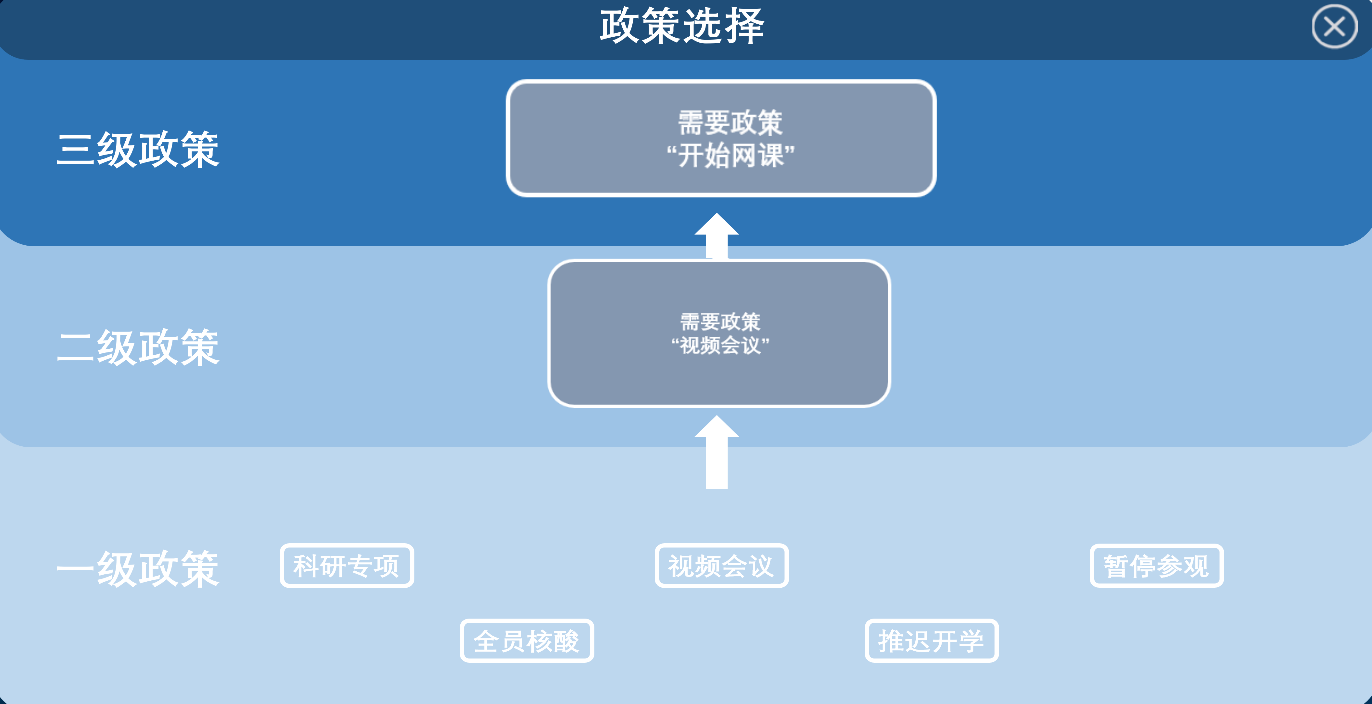
\includegraphics[width=0.9\textwidth]{police_choice.png}
    \caption{学校政策}
    \label{fig:police_choice}
\end{figure}

除此之外,玩家也会遇见一些\textit{事件},玩家可以根据这些\textit{事件}来决定自己的\textit{政策}等。

\begin{figure}[h]
    \centering
    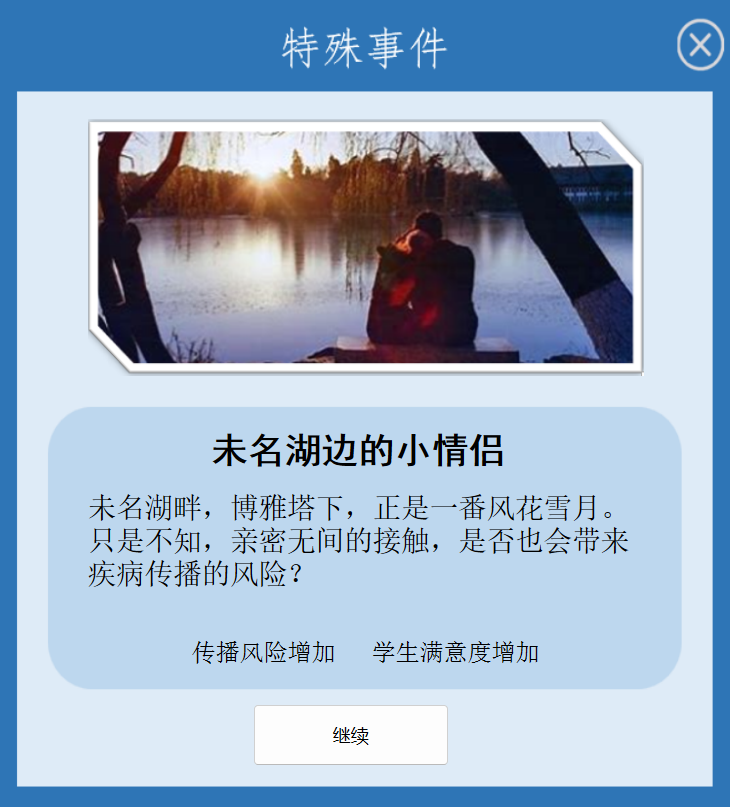
\includegraphics[scale=0.7]{sj.png}
    \caption{事件“未名湖边的小情侣”}
\end{figure}

\section{项目各模块与类设计细节}
我们主要分为两块部分,一是\textit{底层代码},二是\textit{前端}。其中\textit{底层代码}由\textbf{吕杭州}和\textbf{田一阳}负责,而\textit{前端}由\textbf{陈天乐}负责。

\subsection{底层代码}
根据面向对象的编程思想,\textit{底层代码}的实现主要是设计各种\textbf{类}。我们为这个游戏设计了5个主要的基类,分别是用来控制整个主游戏的\texttt{Game}类、代表学校里人员的\texttt{Person}类、代表各种政策的\texttt{Policy}类、代表学校内各种建筑的\texttt{Building}类和代表各类事件的\texttt{Affair}类。
\subsubsection{\texttt{Game}类}
因为这个游戏是基于个体行为模拟的传染病模型,所以在\texttt{Game}类中含有代表所有人员的数组\texttt{all\_person[]},代表着校园里的所有人员。这个类同时还含有校园里的所有建筑\texttt{all\_building[]}。我们通过对于这些数组的操作来进行整个游戏。

下面是这个类里一些主要的方法:

\begin{enumerate}
    \item \texttt{Game::Game();} 这是这个类的初始化,由于类的成员变量繁多,这个函数比较复杂,主要有\textbf{田一阳}完成。
    \item \texttt{void Game::gameRun();} 这是让游戏开始运行,在最初随机选择一位作为零号感染者主要由\textbf{田一阳}完成。
    \item \texttt{int Game::start\_newday();} 这是进行一天的活动,也就是让病毒开始传播,同时让各种事件和政策生效,这主要由\textbf{吕杭州}和\textbf{田一阳}完成。
    \item \texttt{void Game::save(int i);}和\texttt{void Game::load(int i);} 这是游戏的存档和读档功能,主要由\textbf{陈天乐}完成。
    \item \texttt{void Game::startSpread();}和\texttt{void Game::startQuarantine();} 它们分别是模拟病毒传播和模拟隔离,主要由\textbf{吕杭州}完成。
\end{enumerate}

\subsubsection{\texttt{Person}类}
这是对校园里个体的模拟,主要由\textbf{田一阳}实现。个体的满意度会影响到整体的满意度,而整体的满意度又会导致传播概率的变化,因此保持个体的满意度也是非常重要的一件事情。同时一个人一天24小时各有行动轨迹,通过一个人在每个时刻位置的变化可以大致地模拟学校里人员的流动。而一个人被感染或是被隔离,他所居住的建筑被封闭之类,也会导致他一天的轨迹的改变。
\subsubsection{\texttt{Policy}类}
这里面有\textit{建筑政策}和\textit{学校政策},其中\textit{建筑政策}主要由\textbf{吕杭州}实现,\textit{学校政策}主要由\textbf{田一阳}实现。\textit{建筑政策}可能会对整体传播概率和建筑内的传播概率有影响,同时也会影响到人员的\textit{满意度}。

\begin{verbatim}
    // 这些是建筑政策
    class RequireMasks; // 佩戴口罩
    class MeasureTemperatureAndScanCode; // 测温扫码
    class ShutDownBuilding; // 关闭建筑
    class AddBaffle; // 增设挡板
    class StopDineIn; // 停止堂食
    class TemporaryLockdown; // 临时关闭
    class ShutDownDormitory; // 关闭寝室
    // 这些是学校政策
    class Do_pcr; // 全员核酸
    class ReseachOnVirus; // 开始调查研究
    class SuspendCampusTour; // 停止校园参观
    class PostponeStartOfSchool; // 推迟开学
    class ProvideDesktopVideo; // 提供桌面视频会议
    class StartOnlineCourse; // 开始网课
    class StartPF; // 开始PF制
\end{verbatim}

\subsubsection{\texttt{Building}类}
这些建筑主要由\textbf{田一阳}和\textbf{吕杭州}完成。一个建筑要承担人员的来往,同时建筑内人员密度过大又会导致传播概率的增加,而建筑会为我们提供行动点数,等等。所以建筑在这个游戏里承担着重要的角色。
\begin{verbatim}
    // 这些是主要实现的建筑
    class Hospital; // 医院
    class Library; // 图书馆
    class Gate; // 大门
    class Laboratory; // 实验室
    class Dormitory; // 宿舍
    class TeachingBuilding; // 教学楼
    class Playground; // 操场
    class Gymnasium; // 体育馆
    class DiningHall; // 餐厅
    class Lake; // 未名湖
\end{verbatim}

\subsubsection{\texttt{Affair}类}
这些事件主要由\textbf{吕杭州}实现。特殊事件的发生会使得游戏的发展不那么“平稳”,也让游戏节奏更富有变化,这也是我们设计这么多特殊事件的初衷,同时也能更好地将我们的日常生活融入游戏中。事实上,这些事件的文案和图片都是我们精心将当前的学习和生活相结合得到的,希望玩家能在其中找到一些熟悉感。
\begin{verbatim}
    class CoupleByLake; // 未名湖边的小情侣 0 Lake
    class ReadByLake; // 未名湖畔好读书 1 Lake
    // 2号事件是全员核酸检测后触发,只有输出,在输出部分已经由 陈天乐 实现,故空出
    class OnlineExhibition; // 线上展览 3 Library
    class NastyMeals; // 难以下咽的饭菜 4 DiningHall
    class LuxuriousIsolationConditions; // 豪华隔离条件 5 Hospital
    class InterestingQurantineLife; // 有趣的隔离生活 6 Hospital
    class BrokenWashingMachine; // 坏掉的洗衣机 7 Dormitory
    class BrokenAirConditioner; // 坏掉的空调 8 Dormitory
    class BrokenWaterHeater; // 坏掉的热水器 9 Dormitory
    class Gathering; // 家园门口的聚集 10 DiningHall
    class ProtesetInShudong; // 树洞里的抗议 11 All Building
    class SingInDormitory; // 宿舍楼里的歌剧魅影 12 Dormitory
    class ShushuBegins; // “鼠鼠”文学的泛滥 13 Dormitory
    class QuarrelInDormitory; // 宿舍楼里的争吵 14 Dormitory
    class UnbearableSnoring; // 难以忍受的打呼噜声 15 Dormitory
    class Top10InBathroom; // 浴室里的十佳 16 Dormitory
    class LearningInDormitory; // 宿舍里的自习室 17 Dormitory
    class MahjongInDormitory; // 宿舍里的麻将馆 18 Dormitory
    class HarmoniousDormitory; // 和谐的寝室 19 Dormitory
    class HealthySleeping; // 健康的睡眠 20 Dormitory
    class BrokenOutPersonnel; //员工开始崩溃 21 Hospital Library TeachingBuilding DiningHall
    class VolunteerLack; // 基层志愿者人手短缺 22 Hospital
    class LackOfMedicalResources; // 医疗资源短缺 23 Hospital
    class GreatPrevention; // 井然有序的防控 24 Hospital
    class Detention; // 处分! 25 Gate
    class Top10; // 十佳 26 Gymnasium
    class BrokenHeater; // 暖气!该死的暖气坏了! 27 Dormitory
\end{verbatim}

\subsection{前端}
前端的工作主要由陈天乐负责。因为工程量不大而且只有三人合作,所以没有做专门的接口类。同时为了方便窗口的外观设计,以及为了实现不同窗口的不同功能,每一个不同功能的窗口都设计了一个类。主要设计的类有:

\begin{verbatim}
    mainw 核心游戏界面窗口
    widget 起始窗口
    video 用于播放视频的窗口
    save_and_load 用于存档/读档的窗口
    menu 菜单窗口
    tutor 教程窗口
    buildings 建筑选择/升级界面
    build_info 建筑信息显示界面
    policy 政策选择界面
    pchoice 政策升级界面
    event_ 随机事件显示界面
    note 提示框窗口
\end{verbatim}
下面主要对其中比较特别的设计做一些简要说明。

\subsubsection{\texttt{mainw}类}
这个类是核心的游戏界面窗口,它主要有三个功能。一是提供图形交互界面,使玩家与程序进行交互;二是管理其它所有窗口,控制其它窗口的生存周期;三是一定程度上起到接口的作用。

首先交互界面方面,主要是使用\texttt{QPushButton}来实现交互,通过修改\texttt{QPushButton}的样式表来改变\textit{正常情形/鼠标悬停/鼠标按下}时按钮的外观,提高交互体验。右侧利用$\texttt{ScrollAreaWidgetContents}$类做了一个滚动窗口,并且设计函数\texttt{void mainw::a\_text(QString)}在滚动窗口中输出信息。

其中比较独特的设计是,利用一系列的图片素材轮播来实现类似于动画的效果。其中$\texttt{void mainw:: timerun()}$使用\texttt{QTimer}计时,每100ms触发一次\texttt{void mainw::button\_outlook()}来改变按钮外观,从而实现近似于动画的效果。

\begin{figure}[h]
    \centering
    
\includegraphics[width=0.9\textwidth]{timeRun.png}
    \caption{\texttt{timeRun}实现效果图}
\end{figure}

而对于界面最上方感染人数的显示,我们没有使用\texttt{Qt}原生的类,而是使用三个\texttt{QLabel}来实现的,分别是一个中间透明的\textit{“进度槽”},和两个纯色图片来代表\textit{“感染人数”}和\textit{“隔离人数”}。空的槽位放在顶端来遮罩两个纯色图片,每次感染人数变化时,通过计算算出两个纯色图片的长度,从而实现进度槽的效果。

\begin{figure}[h]
    \centering
    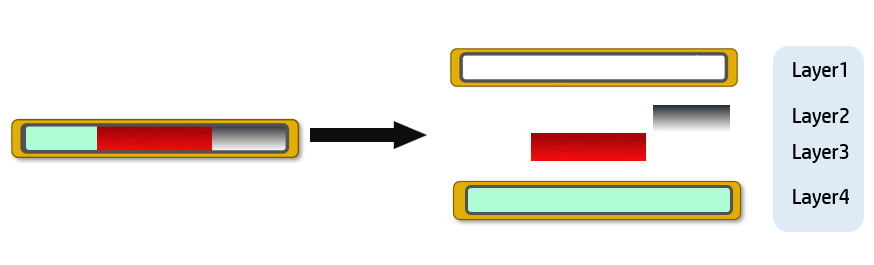
\includegraphics[width=0.9\textwidth]{jinducao.png}
    \caption{进度条效果图}
\end{figure}

此外,\texttt{mainw}还使用了\texttt{Qt}的鼠标点击事件,来控制游戏结束时单击返回开始界面;使用了\texttt{QSoundEffect}来播放音效和背景音乐。

其次\texttt{mainw}有管理其它窗口的功能。\texttt{mainw}中有指向所有其它窗口的指针,并且借此控制它们的打开与关闭。此外,\texttt{mainw}中的函数\texttt{mainw::normalize\_x(int x)}和$\texttt{int mainw::normalize\_y(int y)}$通过读取窗口现在的大小信息,来计算组件/子窗口应该出现的位置,为窗口的缩放做了准备。虽然最后这个功能因为美工要求而被删掉了,但是架构本身是允许窗口的缩放的。

最后,\texttt{mainw}还具有一定程度的接口功能,\texttt{mainw}有指向后端的核心类\texttt{Game}的指针,同时\texttt{Game}也有指向\texttt{mainw}的指针,前后端的数据流通主要就是通过\texttt{mainw}来进行交互的。例如当随机事件发生时,后端会调用$\texttt{void mainw::e\_happen(int idx)}$告诉\texttt{mainw}发生了序号为\texttt{idx}的事件,随后\texttt{mainw}再调动\texttt{event\_}窗口来显示相关事件。

\subsubsection{\texttt{video}类}

\texttt{video}类主要负责动画的播放。在这个程序中体现为:开始动画,游戏结束胜利动画和游戏结束失败动画。因为三种情形下需要实现的功能不同,所以在\texttt{video}构造函数中有\texttt{state}这一参数,来使\texttt{video}获得不同的功能。

例如游戏开始时的“按任意键进入游戏”,就是使用\texttt{Qt}的键盘事件和鼠标事件来实现的。键盘/鼠标按下时首先判断动画是否播放完毕,如果播放完毕,那么就会播放下一段进入游戏开始界面的动画。

\subsubsection{\texttt{note}类}

\texttt{note}类用于显示一些临时信息,例如在按下按钮时提示“行动力不足”等等。因为实现了随时间变透明消失的效果,以及很高的复用率,所以也设计成了一个类。

\texttt{note}类的主要方法是,在\texttt{note}显示后,使用\texttt{QTimer}进行计时,不断触发\texttt{OnTimerTimeout()}这一槽函数,来不断调整窗口透明度。从而实现提示窗口逐渐消失的效果。

\begin{figure}[h]
    \centering
    
\includegraphics{fade.png}
    \caption{窗口逐渐消失效果图}
\end{figure}

此外,这个类还重载了构造函数:

\begin{verbatim}
    void note(QWidget *parent, int c, const int delay_ms = 2000);
    void note(QWidget *parent, QString c, const int delay_ms = 2000);
\end{verbatim}

前者用于便捷地显示\textit{此操作需要行动力c点},而后者用于在窗口中显示其它的文字提示。第一种情况的应用尤其多,为了实现更好的代码复用,做了这样的重载。

\subsubsection{其它类与素材来源}

其它的类主要都是为了实现更多交互内容和更好的显示而设计的。实现方法上大同小异,这里不做赘述。

素材的主要来源有几个部分:音频素材主要来自于网络,图片素材部分来自网络,一部分是实拍并且进行了一定程度的后期处理,视频素材主要是使用自己录制和来自网络的素材剪辑而成的,同时失败动画和成功动画使用了\textit{AI}进行人声配音。


\section{项目总结与反思}
\subsection{总结}
本次合作最值得感谢的是我们共同的努力,先是在二教518的思想碰撞,从刘慈欣的《纤维》到橙光游戏,再从《西厢记》《长生殿》到如今的《continuous》,那个晚上我们是碰撞了如此多的火花,真的非常感谢大家。

然后要感谢的是我们行动力极强的组长\textbf{陈天乐}。他定下的任务自己总是最先完成,甚至有时候会反过来帮助组员们的工作。他也总是和老师、助教及时地沟通,真的非常感谢我们的组长。

最后要感谢的是我们的组员,不摆烂,不失踪,积极参与讨论和编程,积极提供素材,并且及时地完成组长布置的工作。真的是组长和组员的共同努力,才可以使这次合作较为圆满地完成。



\subsection{反思}
在本次合作中,最突出的问题居然是编码问题。由于各个编辑器的不同,以及互相存储打开的编码方式各不相同,导致最后我们的代码里出现了一堆乱码,例如下面就是很典型的一段乱码注释:
\begin{verbatim}
    bool MeasureTemperatureAndScanCode::available() {
    // ÿ��������ж�������2
    // ��ǰ�Ƕ����������Ϳ��Բ����������
    // 上面这堆乱码应该是显示不出来的
    if (BuildingAttached()->getLevel() >= 2)
        return true;
    return false;
}
\end{verbatim}

其次是我们的变量和方法命名问题,我们初始没有设计好一个较好的命名规范,只是在\textbf{吕杭州}和\textbf{田一阳}之间有一个简单的口头约定,而这个约定也很快在实践中被抛之脑后,导致我们的变量和方法命名千奇百怪、五花八门,这也是以后值得注意的问题。

另外我们对于\texttt{Github}的代码托管和版本控制也利用的较差,基本上依靠微信进行版本更新和文件传输,这也是较为薄弱的地方。


\section{结语}

非常感谢你能读到这个文档的末尾,通过这次程序设计实习的课程大作业,我们小组每个人都学到了许多,\texttt{Qt}的使用、面向对象编程、\LaTeX 的使用、软件开发需要的种种合作技能等,但是最重要的是我们之间连续不断的友谊。

最后,非常感谢程序设计实习给予我们这次机会挑战自己,也愿程序设计实习这门课越办越好,愿助教们工作顺利、学业有成,也祝愿\textbf{郭炜、张勤健、刘家瑛}老师\texttt{paper++、happiness++}!

\begin{flushright}
    zokuzoku小组 \\
    2023年7月4日夜
\end{flushright}
    

\end{document}